\documentclass[12pt]{article}

% 页面设置
\usepackage{geometry}
\geometry{left=2.5cm, right=2.5cm, top=2.5cm, bottom=2.5cm}  % 设置页边距
\usepackage{graphicx}  % 引用图片
\usepackage{ctex}
\usepackage{fontspec}
\usepackage{setspace}

% 字体设置
\setmainfont{Times New Roman}
\setCJKmainfont{SimSun}
\setCJKsansfont{SimHei}

% 表格设置
\usepackage{makecell}
\newcommand{\addcell}[2][4]{\makecell{\zihao{#1}\textsf{#2}}}
\usepackage{titlesec}
\usepackage{booktabs}
\usepackage{tabularx}

% 设置图注、表注
\usepackage{caption}
\usepackage{bicaption}
\captionsetup{labelsep=quad, font={small, bf}, skip=2pt}
\DeclareCaptionOption{english}[]{
    \renewcommand\figurename{Fig.}
    \renewcommand\tablename{Table}
}
\captionsetup[bi-second]{english}

% 设置页眉
\usepackage{fancyhdr}
\pagestyle{fancy}
\fancypagestyle{preContent}{
    \fancyhead[L]{\zihao{-5} 物理化学实验}
    \fancyhead[C]{\zihao{-5} 实验4\ \ 双液体系沸点-成分图的绘制}
    \fancyhead[R]{\zihao{-5} 1800011716\ 王崇斌}
}
\pagestyle{preContent}

%	设置首页页眉页脚
\fancypagestyle{plain}{
	\fancyhead[L]{\zihao{-5} 物理化学实验}
	\fancyhead[C]{\zihao{-5} 实验4\ \ 双液体系沸点-成分图的绘制}
	\fancyhead[R]{\zihao{-5} 1800011716\ 王崇斌}
	\cfoot{}
}

% 设置标题格式
\titleformat*{\section}{\zihao{4}\sffamily}
\titleformat*{\subsection}{\zihao{-4}\sffamily}
\titleformat*{\subsubsection}{\zihao{-4}\sffamily}
\titlespacing*{\section}{0pt}{10pt}{10pt}
\titlespacing*{\subsection}{0pt}{10pt}{5pt}
\titlespacing*{\subsubsection}{0pt}{10pt}{5pt}

% 设置引用格式
\usepackage[super,round,comma,compress]{natbib}
\usepackage{hyperref}  % 使用hyperref包,可以提供文献引用到文件末尾


% 一些相关的包
\usepackage{amsmath}  % 数学公式
\usepackage{amssymb}  % 特殊字符
\usepackage[version=4]{mhchem}  % 用于输入化学式
\usepackage{braket}  % 用于输入Dirac符号
\usepackage{subfigure}  % 多张图片的排版

% 定义常用的命令
\def\d{\mathrm{d}}  % 正体的常用数学常数
\def\e{\mathrm{e}}
\def\i{\mathrm{i}}
\def\dps{\displaystyle}  % 
\newcommand{\mr}[1]{\mathrm{#1}}
\newcommand{\mb}[1]{\mathbf{#1}}
\newcommand{\dv}[2]{\frac{\d{#1}}{\d{#2}}}  % 定义导数、偏导数的简便记号
\newcommand{\pdv}[2]{\frac{\partial{#1}}{\partial{#2}}}
\def\degree{$^{\circ}$}  % 角度
\def\celsius{^{\circ}\mr{C}}  % 摄氏度

%正文
\begin{document}
    % 标题页
    \begin{titlepage}
    	% 页眉
    	\thispagestyle{plain}
        % 图片
        \begin{figure}[h]
            \centering
            \includegraphics{pku.png}
        \end{figure}
        \vspace{24pt}
        % 标题
        \centerline{\zihao{-0} \textsf{物理化学实验报告}}
        \vspace{40pt} % 空行
        \begin{center}
            \begin{tabular}{cp{14.1cm}}
                % 题目
                \addcell[2]{题目:\ } & \addcell[2]{双液体系沸点-成分图的绘制} \\
                \cline{2-2}
            \end{tabular}
        \end{center}
        \vspace{20pt} % 空行
        \begin{center}
            \doublespacing
            \begin{tabular}{cp{5cm}}
                % 姓名
                \addcell{姓\phantom{空格}名:\ } & \addcell{王崇斌} \\
                \cline{2-2}
                % 学号
                \addcell{学\phantom{空格}号:\ } & \addcell{1800011716}\\
                \cline{2-2}
                % 组别
                \addcell{组\phantom{空格}别:\ } & \addcell{19组} \\
                \cline{2-2}
                % 实验日期
                \addcell{实验日期:\ } & \addcell{2021.09.30}\\
                \cline{2-2}
                % 室温
                \addcell{室\phantom{空格}温:\ } & \addcell{296.96\ K}\\
                \cline{2-2}
                % 大气压强
                \addcell{大气压强:\ } & \addcell{100.02\ kPa}\\
                \cline{2-2}
            \end{tabular}
            \begin{tabular*}{\textwidth}{c}
                \\ % 这是空行
                \\ % 这是空行
                \\ % 这是空行
                \\ % 这是空行
                \hline % 分割线
            \end{tabular*}
        \end{center}
        % 摘要
        \textsf{摘\ \ 要}\ \ 本实验通过改变液相组分,利用回流冷凝法测定气液两相达到平衡时的沸点
		,同时收集气液两相的混合物,测定折射率,与绘制的标准工作曲线比较,确定气液两相的组成,进一步绘制出
		乙醇-环己烷双液体系的沸点-成分图。通过相图确定了这个体系的最低恒沸点为$64.20\celsius$,此时液相
		乙醇质量分数$w_{\mr{EtOH}}=0.324$,与文献有一定差异,分析了误差产生的原因。
        \\
        \\
        % 关键字
        \textsf{关键词}\ \ 最低恒沸点,组成-沸点图,阿贝折射仪
    \end{titlepage}
	\vbox{}        
    \section{实验部分}
    	\subsection{仪器和试剂}
		\begin{enumerate}
			\item 试剂:环己烷(AR)、无水乙醇(AR)
			\item 仪器:恒沸点仪,恒温器,阿贝折射仪,电阻丝,1/10刻度温度计,移液管,滴瓶等
		\end{enumerate}
		\subsection{实验内容}
			\subsubsection{沸点和两相成分的测定}
			\begin{figure}[h]
				\centering
				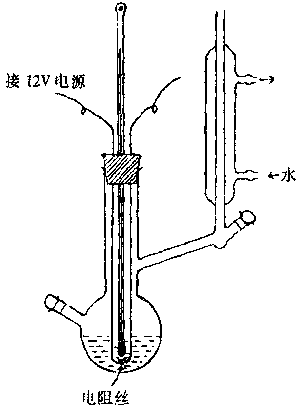
\includegraphics[width=0.25\textwidth]{device.png}
				\bicaption{恒沸点仪}{Experimental Device of Constant Boiling Point}
				\label{exp device}
			\end{figure}
			\par 
			实验装置如图\ref{exp device}所示。向蒸馏瓶中加入20mL乙醇,温度计水银球1/2浸入液体内。
			将电阻丝连接变压器,加热蒸馏瓶内液体直到完全沸腾,待温度稳定后记录温度计读数与大气压。
			切断电源后分别取支管处的气相冷凝液和蒸馏瓶中的液体几滴,测定折射率
			\footnote{注意阿贝折射仪要连接恒温器,本实验中所有折射率的测定都在30$\celsius$下进行}
			,重复三次并计算平均值
			\footnote{事实上这是实验书上叙述的步骤,在真实的操作中只测定了一次,另外两次纯乙醇
			折射率的测定使用了试剂瓶中的乙醇}
			。
			\par
			向蒸馏瓶中加入1mL环己烷,按上述方法测其沸点及气、液两相折射率(只读一
			次数)。再依次分别加入1mL、2mL、3mL、4mL、3mL、5mL环己烷
			\footnote{由于操作者的疏忽,与实验书上的要求有一点偏差}
			,作同样实验。
			\par 
			在上述实验结束后,将蒸馏瓶内母液回收,用少量环己烷清洗蒸馏瓶3-4次,加入20ml环己烷,装好仪器。
			先测定环己烷的沸点,然后依次加入0.2mL、0.2mL、0.5mL、0.5mL、2 mL、5mL、5mL乙醇,
			分别测定它们的沸点及气、液两相样品的折射率。
			\subsubsection{标准工作曲线的绘制}
			配置不同比例(见“数据与结果”部分)的乙醇-环己烷混合溶液,用差量法分别得到其中乙醇与环己烷的质量,
			进而得到质量分数,在恒温下分别测定这些样品的折射率。
	\vbox{}  
	\section{数据与结果}
 		\subsection{沸点和两相成分测定}
		\par 
		向乙醇中加入环己烷时折射率变化数据如表\ref{add CyH to EtOH n}。
 		\begin{table}[h]
 			\centering
 			\zihao{5}
 			\bicaption{向乙醇中加入环己烷的沸点与气液相折射率数据表}{Refractive Index and b.p. Data (Adding CyH to EtOH)}
 			\begin{tabular}{cccc}
 				\toprule
				$V_{add}$(CyH)/mL & $n_{g}$ & $n_l$ & $T_b/\celsius$ \\
 				\midrule
				0  & 1.3585 & 1.3587 & 77.40 \\
				1  & 1.3737 & 1.3615 & 74.10 \\
				2  & 1.3798 & 1.3630 & 72.05 \\
				4  & 1.3889 & 1.3658 & 69.10 \\
				7  & 1.3919 & 1.3721 & 66.83 \\
				11 & 1.3962 & 1.3774 & 65.50 \\
				13 & 1.3975 & 1.3804 & 65.00 \\
				19 & 1.3986 & 1.3853 & 64.60 \\
 				\bottomrule
 			\end{tabular}
			 \label{add CyH to EtOH n}
 		\end{table}
		\par 
		向环己烷中加入乙醇时折射率变化如表\ref{add EtOH to CyH n}。
		\begin{table}[h]
			\centering
			\zihao{5}
			\bicaption{向环己烷中加入乙醇的沸点与气液相折射率数据表}{Refractive Index and b.p. Data (Adding EtOH to CyH)}
			\begin{tabular}{cccc}
				\toprule
			   $V_{add}$(EtOH)/mL & $n_{g}$ & $n_l$ & $T_b/\celsius$ \\
				\midrule
			   0.0  & 1.4219 & 1.4219 & 79.62 \\
			   0.2  & 1.4029 & 1.4204 & 77.45 \\
			   0.4  & 1.4010 & 1.4186 & 73.15 \\
			   0.9  & 1.4000 & 1.4148 & 67.10 \\
			   1.4  & 1.3996 & 1.4159 & 65.40 \\
			   3.4  & 1.3993 & 1.4089 & 64.30 \\
			   8.4  & 1.3984 & 1.3985 & 64.20 \\
			   13.4 & 1.3985 & 1.3910 & 64.30 \\
				\bottomrule
			\end{tabular}
			\label{add EtOH to CyH n}
		\end{table}
 		\vbox{}

 		\subsection{标准工作曲线的绘制}
		\par 
		由于不同实验者的阿贝折射仪有着不同的系统误差,因此需要绘制标准工作曲线来消除这种误差对测量的影响。
		表 中记录了标准样品的配比信息(测定滴瓶的增重来确定加入乙醇和环己烷的量)和该实验者使用的阿贝折射仪
		测量的折射率数据。
		\begin{table}[h]
			\centering
			\zihao{5}
			\bicaption{标准工作曲线数据表}{Data of Standard Working Curve}
			\begin{tabular}{cccccccc}
				\toprule
			    编号 & 1 & 2 & 3 & 4 & 5 & 6 & 7 \\
				\midrule
				$V_{\mr{EtOH}}/V_{\mr{CyH}}$ & 1 / 7 & 2 / 6 & 3 / 5 & 4 / 4 & 5 / 3 & 6 / 2 & 7 / 1 \\
				$m_0$(空瓶质量)/g & 28.2617 & 85.2854 & 33.0748 & 35.3946 & 40.3717 & 32.5840 & 32.8031 \\
				$m_1$(+EtOH)/g & 29.7975 & 86.8342 & 35.4198 & 38.5233 & (+CyH)42.6743 & 37.2544 & 38.2999 \\
				$m_2$(+CyH)/g & 40.1528 & 91.4171 & 39.2612 & 41.5876 & (+EtOH)46.5056 & 38.7883 & 39.0683 \\
				$m_{\mr{EtOH}} = m_1 - m_0$ /g & 1.5358 & 1.5488 & 2.3450 & 3.1287 & 3.8322 & 4.6704 & 5.4968\\
				$m_{\mr{CyH}} = m_2 - m_1$ /g & 10.731 & 4.5892 & 3.8414 & 3.0653 & 2.3026 & 1.5339 & 0.7684 \\
				$w_{\mr{EtOH}} = \dfrac{m_{\mr{EtOH}}}{m_{\mr{CyH}} + m_{\mr{EtOH}}}$ &  0.12520 & 0.25233 & 0.37906 & 0.50512 & 0.62466 & 0.75277 & 0.87735\\
				$n_1$ & 1.4136 & 1.4039 & 1.3949 & 1.3861 & 1.3774 & 1.3705 & 1.3640 \\
				$n_2$ & 1.4134 & 1.4040 & 1.3950 & 1.3858 & 1.3775 & 1.3706 & 1.3639 \\
				$n_3$ & 1.4133 & 1.4040 & 1.3950 & 1.3860 & 1.3776 & 1.3703 & 1.3641 \\
				$\bar{n}$ & 1.4134 & 1.4040 & 1.3950 & 1.3860 &	1.3775 & 1.3705 & 1.3640 \\
				\bottomrule
			\end{tabular}
			\label{standard curve}
		\end{table}
		将上述表格中折射率-$w_{\mr{EtOh}}$作图,可以从图\ref{standard w c}中看到,线性回归并不能很好地描述两者之间的关系,
		虽然有着很高的相关系数(-0.9979),但是数据明显呈现出“凸”的性质。因此考虑用二次曲线拟合,结果为
		图中蓝线所示,效果较好。拟合得到的标准工作曲线的表达式为:
		\begin{equation}
			n = 0.01830w^2 - 0.08479w + 1.42402809
			\label{working eq}
		\end{equation}
		\begin{figure}[htbp]
			\centering
			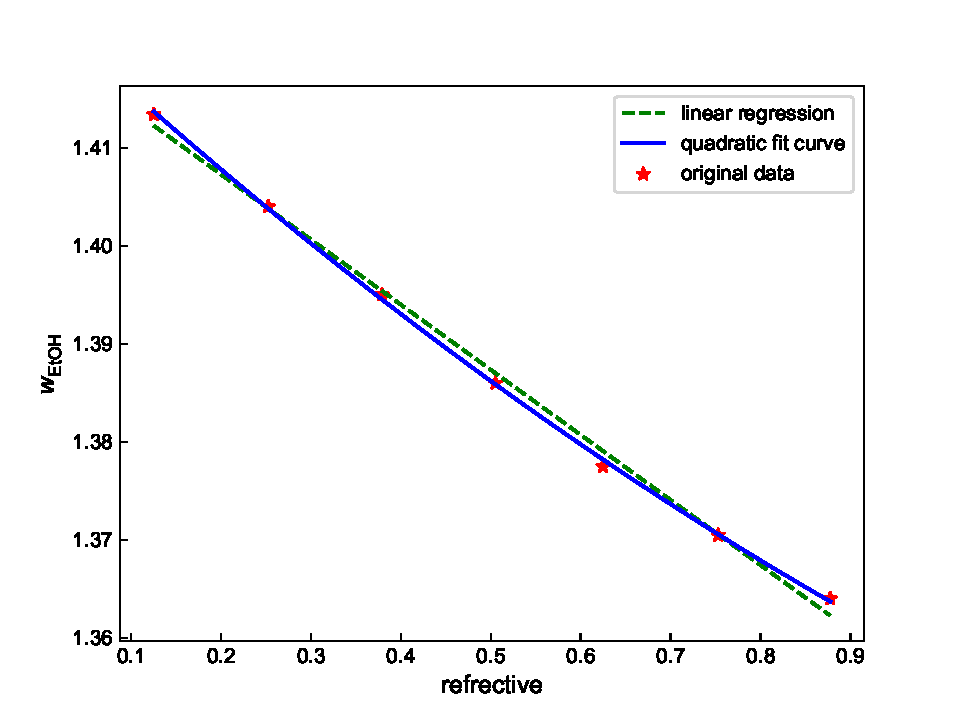
\includegraphics[scale=0.7]{working_curve.pdf}
			\bicaption{标准工作曲线}{Standard Working Curve}
			\label{standard w c}
		\end{figure}
 		\subsection{气液平衡相图的绘制}
		\par 
		首先根据拟合的曲线得到实验中气液两相的组成(需要解一元二次方程\ref{working eq}),现在将沸点与组成的数据列于表\ref{working curve table}。
		\begin{table}[h]
			\centering
			\zihao{5}
			\bicaption{沸点与气、液相中乙醇含量的关系表}{the Relation Between b.p and $w_{\mr{EtOh}}$}
			\begin{tabular}{cccccc}
				\toprule
				样本 & 沸点$\celsius$ & $n_g$ & $n_l$ & $w_{\mr{EtOH},g}$ & $w_{\mr{EtOH},l}$\\
				\midrule
				1  & 77.40 & 1.3585 & 1.3587 & 0.9804 & 0.9762  \\   
				2  & 74.10 & 1.3737 & 1.3615 & 0.6991 & 0.9203  \\  
				3  & 72.05 & 1.3798 & 1.3630 & 0.5991 & 0.8913  \\  
				4  & 69.10 & 1.3889 & 1.3658 & 0.4600 & 0.8386  \\ 
				5  & 66.83 & 1.3919 & 1.3721 & 0.4163 & 0.7263  \\  
				6  & 65.50 & 1.3962 & 1.3774 & 0.3555 & 0.6377  \\  
				7  & 65.00 & 1.3975 & 1.3804 & 0.3375 & 0.5896  \\  
				8  & 64.60 & 1.3986 & 1.3853 & 0.3223 & 0.5137  \\  
				9  & 79.62 & 1.4219 & 1.4219 & 0.0252 & 0.0252  \\  
				10 & 77.45 & 1.4029 & 1.4204 & 0.2643 & 0.0432  \\   
				11 & 73.15 & 1.4010 & 1.4186 & 0.2897 & 0.0649  \\   
				12 & 67.10 & 1.4000 & 1.4148 & 0.3032 & 0.1115  \\   
				13 & 65.40 & 1.3996 & 1.4159 & 0.3087 & 0.0979  \\   
				14 & 64.30 & 1.3993 & 1.4089 & 0.3128 & 0.1859  \\   
				15 & 64.20 & 1.3984 & 1.3985 & 0.3251 & 0.3237  \\   
				16 & 64.30 & 1.3985 & 1.3910 & 0.3237 & 0.4293  \\              
				\bottomrule
			\end{tabular}
			\label{working curve table}
		\end{table}
		\par 
		根据这些数据可以绘制气液平衡时的相图\ref{phase diagram},拟合的方法为常用的三次样条插值,
		但是这也造成了一些问题,多项式拟合无法处理突变很快的函数,比如图\ref{phase diagram}的左半边,
		在多次尝试之后,将左半边的液相曲线舍去了一个点,将气相曲线用分段线性插值拟合,得到了相对合理的结果。
		如果对左半部分气相线进行三次样条插值,那么会得到图\ref{phase diagram bad}中所展示的不符合物理的结果。
		\begin{figure}[htbp]
			\centering
			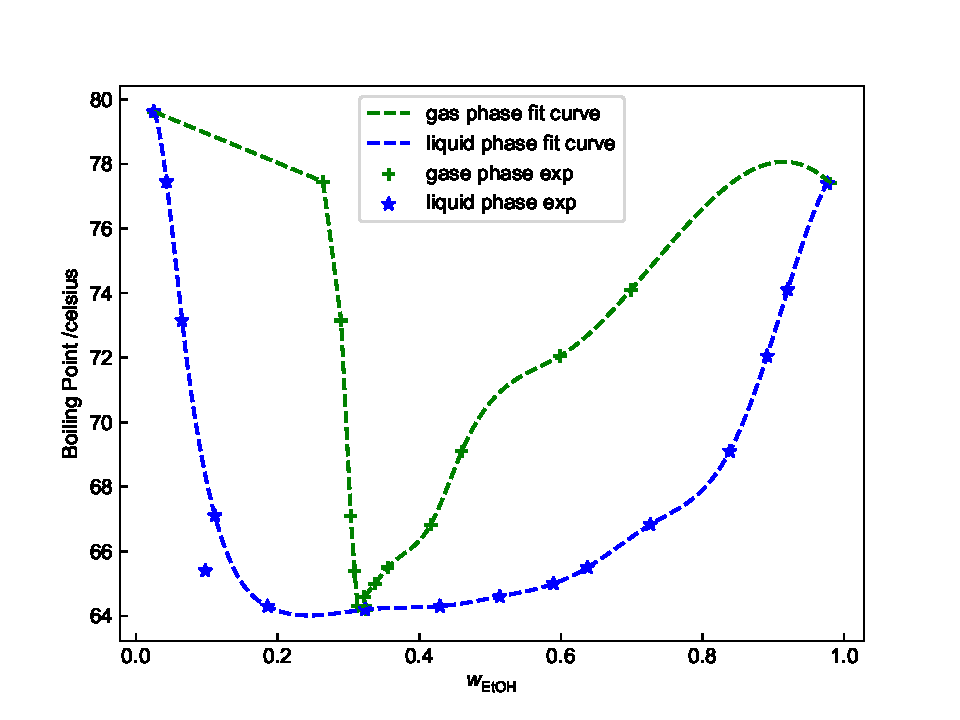
\includegraphics[scale=0.7]{phase_diagram.pdf}
			\bicaption{乙醇-环己烷体系沸点-成分图}{Boiling Point v.s. Phase Composition Diagram}
			\label{phase diagram}
		\end{figure}
		\begin{figure}[htbp]
			\centering
			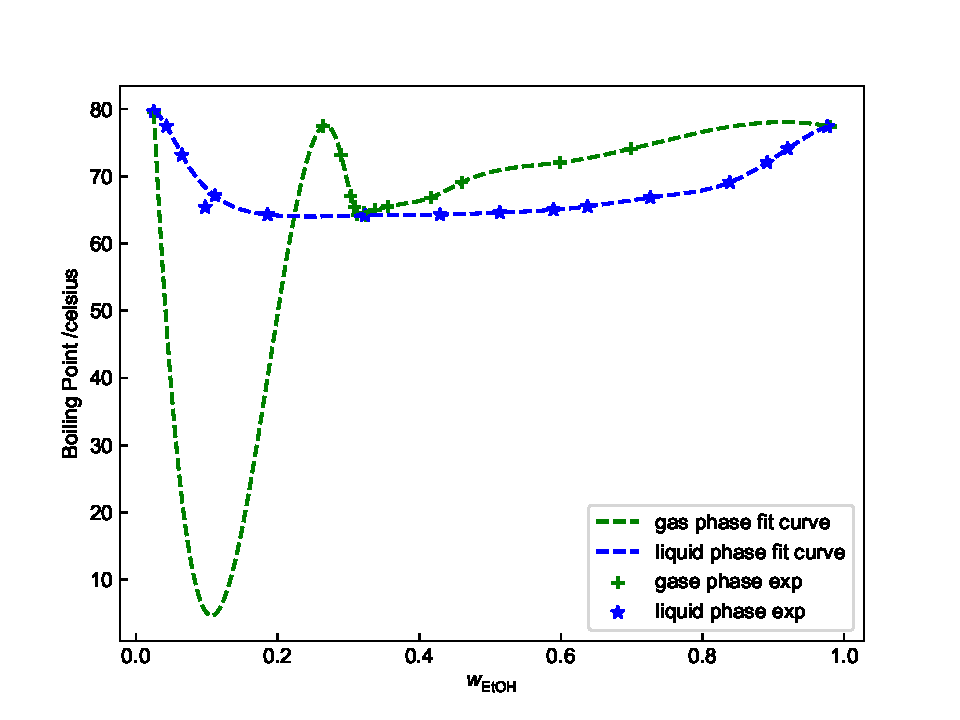
\includegraphics[scale=0.7]{phase_diagram_bad.pdf}
			\caption{失败的拟合结果}
			\label{phase diagram bad}
		\end{figure}
		\par 
		从图\ref{phase diagram}中(或者实验数据表格\ref{working curve table}第15组数据)中都可以直接看出,
		环己烷-乙醇混合物的共沸点在$64.2\celsius$附近。表格\ref{working curve table}第15组数据中
		气液相组成并不完全相同,但是考虑到阿贝折射仪在度数时最后一位的估读误差大约有$\pm0.0001$,那么
		可以认为第15组数据代表了共沸点,此时气液相乙醇的质量分数约等于0.324。
		\vbox{}  	
 	\section{讨论与结论}
		\subsection{实验讨论}
		\subsubsection{实验结果的可靠性}
		查阅参考文献\citealp{doi:10.1021/je60019a024},得知共沸点为$64.77\celsius$,
		共沸时气液相的乙醇摩尔分数为$x_{\mr{EtOH}} = 0.431$,
		转换为质量分数:
		\begin{equation}
			w_{\mr{EtOH}} = \frac{x_{\mr{EtOH}}\cdot M_{\mr{EtOH}}}{x_{\mr{EtOH}}\cdot M_{\mr{EtOH}} + x_{\mr{CyH}}\cdot M_{\mr{CyH}}}
			= 0.293
		\end{equation}
		可以计算本实验中测量值的相对偏差为:
		\begin{equation}
			E_r(T_b) = \dfrac{|T_{b,exp} - T_{b,real}|}{T_{b,real}} = 0.9\%
		\end{equation}
		\begin{equation}
			E_r(w_{\mr{EtOH}}) = \dfrac{|w_{\mr{EtOH},exp} - w_{\mr{EtOH},real}|}{w_{\mr{EtOH},real}} = 10\%
		\end{equation}
		可以清晰地看到共沸点温度与文献值相差并不多但是组成与文献值偏差较大。
		\subsubsection{误差来源的讨论}
		\par 
		首先温度计示数存在系统误差,通过与其他同学对比纯环己烷与纯乙醇沸点测定的数据,我的温度计
		比同组另一个同学尚游皓偏低$0.4\celsius$,因此温度计的示数系统误差\textbf{完全可以}导致实验中共沸点
		温度与文献值的偏差。
		\par 
		共沸点组成与文献值偏差很大,可能的原因有:溶液挥发、阿贝折射仪的度数误差。
		实验中观察到了气相冷凝液在阿贝折射仪上以肉眼可见的速度挥发,因此在测定气相组成的时候,
		乙醇的含量会偏高。由于气液平衡时液相组成在很大温度范围内基本不变,因此气相中乙醇含量
		测量值偏大会严重导致计算共沸点时乙醇含量偏大,但是共沸点的温度几乎不受影响,这或许
		可以解释为何共沸点乙醇含量比文献值大。文献\citealt{doi:10.1021/je60019a024}中列出了
		标准大气压下的沸点-成分图与实验的数据,参见图\ref{phase data paper},\ref{phase diagram paper}。
		\begin{figure}
			\centering
			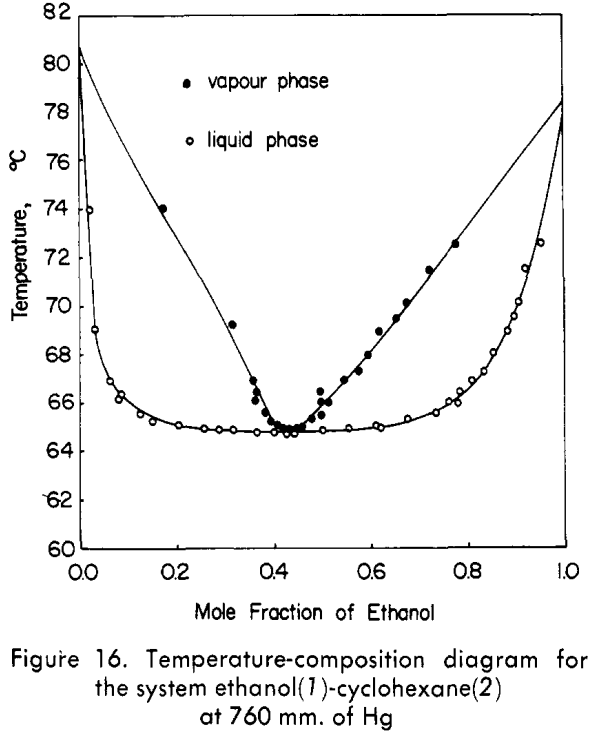
\includegraphics[scale=0.5]{phase_diagram_paper.png}
			\caption{参考文献\citealt{doi:10.1021/je60019a024}中给出的相图}
			\label{phase diagram paper}
		\end{figure}
		\begin{figure}
			\centering
			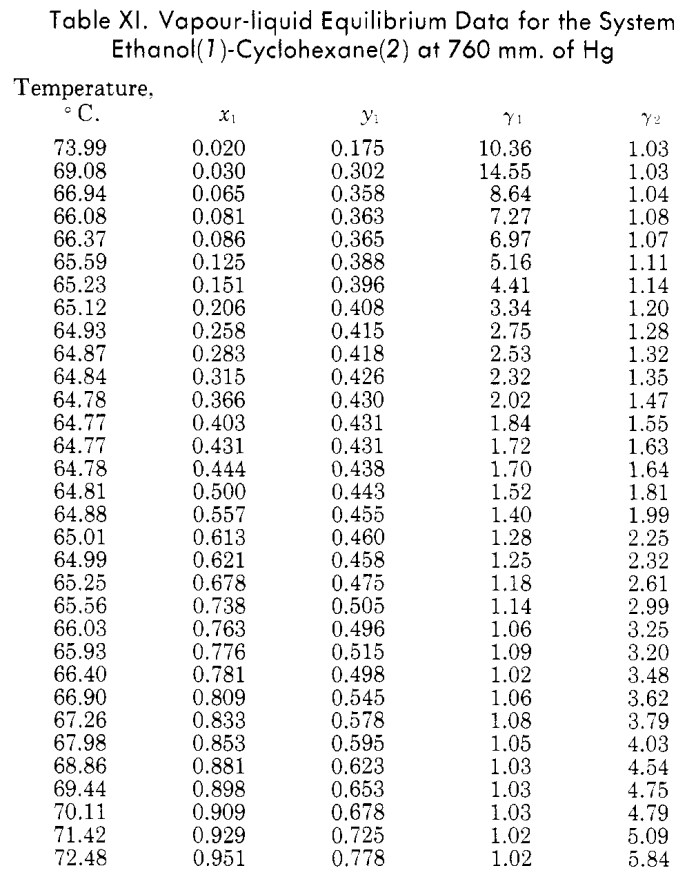
\includegraphics[scale=0.5]{phase_data_paper.png}
			\caption{参考文献\citealt{doi:10.1021/je60019a024}中给出的实验数据点}
			\label{phase data paper}
		\end{figure}
		\par 
		个人认为阿贝折射仪度数的误差并不是主要的,因为度数误差只有$\pm0.0001$,按照线性近似
		的标准工作曲线来估计,这只会对质量分数的测定产生$0.3\%$左右的误差,完全不会累积到
		$10\%$的量级,所以唯一的可能就是放入阿贝折射仪测定的样品本身有误差。
		\par 
		事实上还有一个可能的误差来源,支管处取样的并不一定能代表气液平衡时的气相的成分组成,
		因为升温过程中,在沸点附近,也有可能有大量蒸气冷凝在支管处,导致支管处的液体不能代表平衡时的
		气相组成。实验操作中可以通过在溶液沸腾、温度稳定后倾斜烧瓶将支管处溶液倒回,重新收集溶液的
		方法来减小这种误差。
		\subsection{实验结论}
		本实验采用回流冷凝法测定不同浓度环己烷-乙醇体系的沸点和气液两相折射率,同时
		利用不同浓度环己烷-乙醇标准溶液绘制阿贝折射仪的标准工作曲线,进一步确定两相平衡时
		乙醇的质量分数,绘制出环己烷-乙醇双液体系在大气压下的沸点-成分图,同时确定了这一体系具有
		最低恒沸点64.20$\celsius$,该混合物中乙醇的质量分数为$0.324$,与文献值进行比较,讨论了
		误差的主要来源。
	\vbox{}
	\bibliographystyle{achemso}
	\bibliography{cite}
\end{document}